% Created by tikzDevice version 0.7.0 on 2014-07-29 12:11:08
% !TEX encoding = UTF-8 Unicode
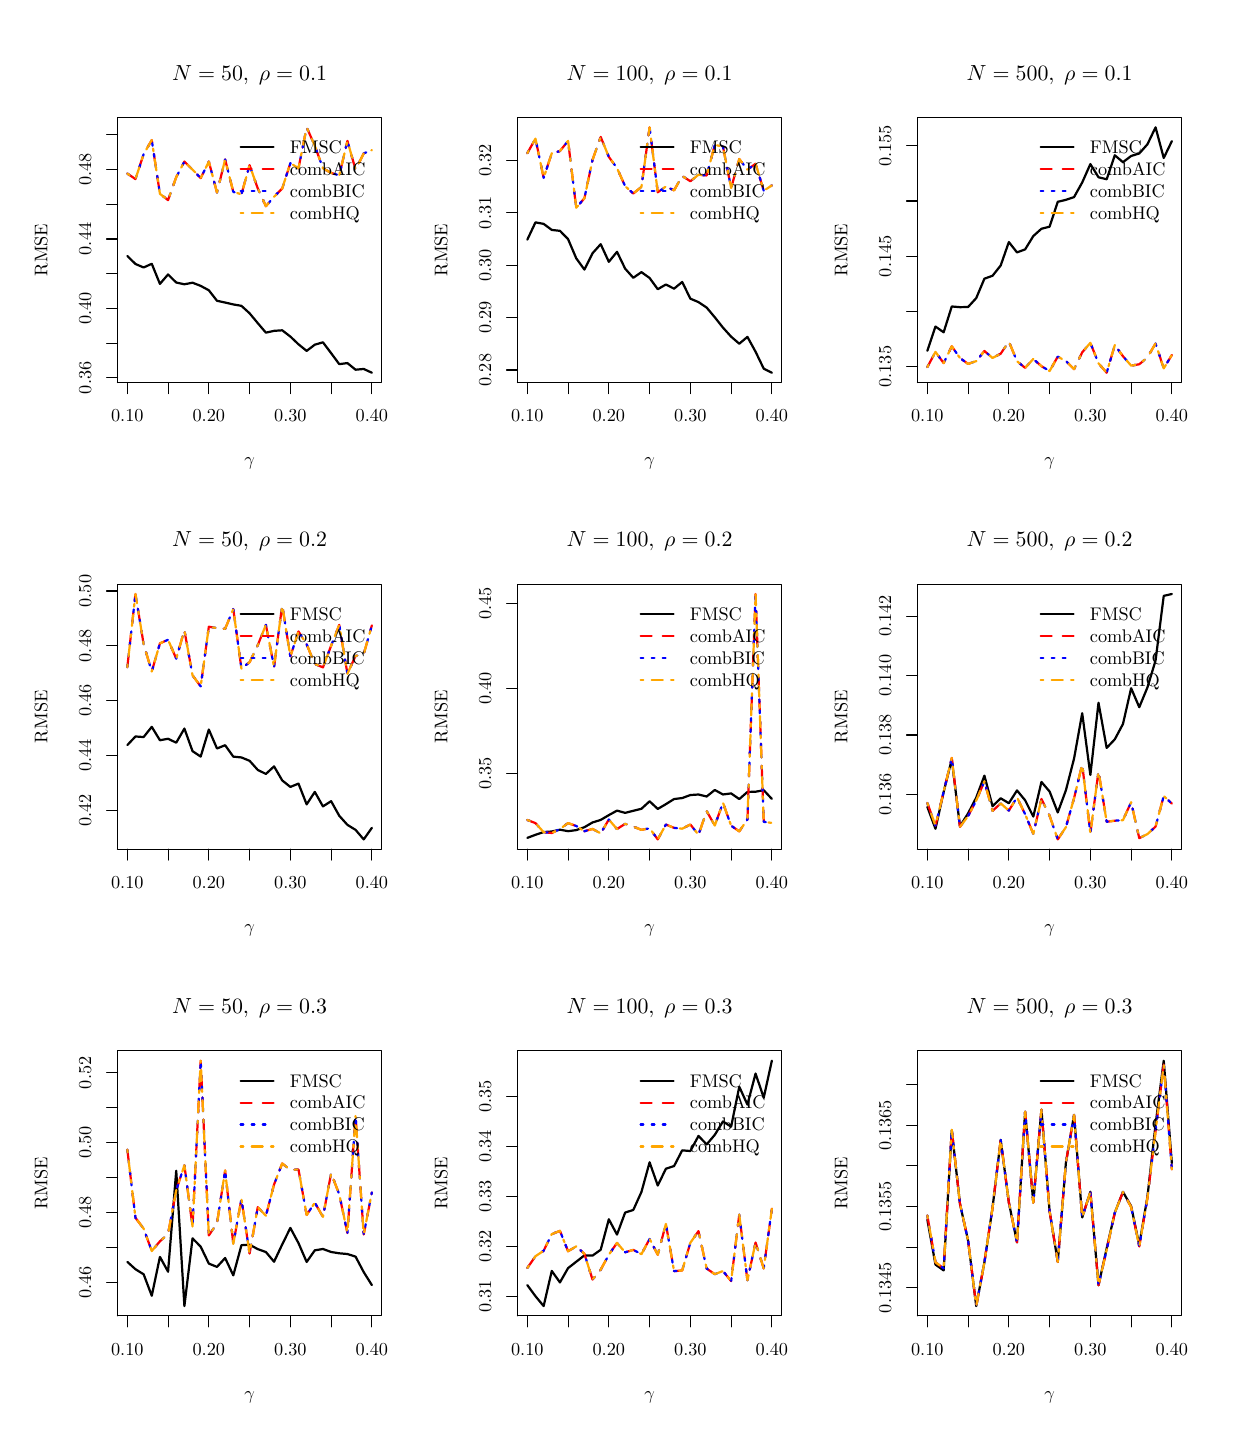
\begin{tikzpicture}[x=1pt,y=1pt]
\definecolor[named]{fillColor}{rgb}{1.00,1.00,1.00}
\path[use as bounding box,fill=fillColor,fill opacity=0.00] (0,0) rectangle (433.62,505.89);
\begin{scope}
\path[clip] ( 32.47,377.65) rectangle (127.91,473.42);
\definecolor[named]{drawColor}{rgb}{0.00,0.00,0.00}

\path[draw=drawColor,line width= 0.8pt,line join=round,line cap=round] ( 36.01,423.38) --
	( 38.95,420.49) --
	( 41.90,419.23) --
	( 44.84,420.56) --
	( 47.79,413.30) --
	( 50.73,416.72) --
	( 53.68,413.79) --
	( 56.63,413.16) --
	( 59.57,413.73) --
	( 62.52,412.58) --
	( 65.46,410.99) --
	( 68.41,407.20) --
	( 71.35,406.56) --
	( 74.30,405.88) --
	( 77.24,405.37) --
	( 80.19,402.67) --
	( 83.14,399.12) --
	( 86.08,395.68) --
	( 89.03,396.33) --
	( 91.97,396.53) --
	( 94.92,394.27) --
	( 97.86,391.47) --
	(100.81,389.09) --
	(103.75,391.33) --
	(106.70,392.19) --
	(109.65,388.27) --
	(112.59,384.30) --
	(115.54,384.69) --
	(118.48,382.29) --
	(121.43,382.56) --
	(124.37,381.20);
\end{scope}
\begin{scope}
\path[clip] (  0.00,  0.00) rectangle (433.62,505.89);
\definecolor[named]{drawColor}{rgb}{0.00,0.00,0.00}

\path[draw=drawColor,line width= 0.4pt,line join=round,line cap=round] ( 36.01,377.65) -- (124.37,377.65);

\path[draw=drawColor,line width= 0.4pt,line join=round,line cap=round] ( 36.01,377.65) -- ( 36.01,373.69);

\path[draw=drawColor,line width= 0.4pt,line join=round,line cap=round] ( 50.73,377.65) -- ( 50.73,373.69);

\path[draw=drawColor,line width= 0.4pt,line join=round,line cap=round] ( 65.46,377.65) -- ( 65.46,373.69);

\path[draw=drawColor,line width= 0.4pt,line join=round,line cap=round] ( 80.19,377.65) -- ( 80.19,373.69);

\path[draw=drawColor,line width= 0.4pt,line join=round,line cap=round] ( 94.92,377.65) -- ( 94.92,373.69);

\path[draw=drawColor,line width= 0.4pt,line join=round,line cap=round] (109.65,377.65) -- (109.65,373.69);

\path[draw=drawColor,line width= 0.4pt,line join=round,line cap=round] (124.37,377.65) -- (124.37,373.69);

\node[text=drawColor,anchor=base,inner sep=0pt, outer sep=0pt, scale=  0.66] at ( 36.01,363.40) {0.10};

\node[text=drawColor,anchor=base,inner sep=0pt, outer sep=0pt, scale=  0.66] at ( 65.46,363.40) {0.20};

\node[text=drawColor,anchor=base,inner sep=0pt, outer sep=0pt, scale=  0.66] at ( 94.92,363.40) {0.30};

\node[text=drawColor,anchor=base,inner sep=0pt, outer sep=0pt, scale=  0.66] at (124.37,363.40) {0.40};

\path[draw=drawColor,line width= 0.4pt,line join=round,line cap=round] ( 32.47,379.34) -- ( 32.47,467.18);

\path[draw=drawColor,line width= 0.4pt,line join=round,line cap=round] ( 32.47,379.34) -- ( 28.51,379.34);

\path[draw=drawColor,line width= 0.4pt,line join=round,line cap=round] ( 32.47,391.89) -- ( 28.51,391.89);

\path[draw=drawColor,line width= 0.4pt,line join=round,line cap=round] ( 32.47,404.44) -- ( 28.51,404.44);

\path[draw=drawColor,line width= 0.4pt,line join=round,line cap=round] ( 32.47,416.99) -- ( 28.51,416.99);

\path[draw=drawColor,line width= 0.4pt,line join=round,line cap=round] ( 32.47,429.54) -- ( 28.51,429.54);

\path[draw=drawColor,line width= 0.4pt,line join=round,line cap=round] ( 32.47,442.08) -- ( 28.51,442.08);

\path[draw=drawColor,line width= 0.4pt,line join=round,line cap=round] ( 32.47,454.63) -- ( 28.51,454.63);

\path[draw=drawColor,line width= 0.4pt,line join=round,line cap=round] ( 32.47,467.18) -- ( 28.51,467.18);

\node[text=drawColor,rotate= 90.00,anchor=base,inner sep=0pt, outer sep=0pt, scale=  0.66] at ( 22.97,379.34) {0.36};

\node[text=drawColor,rotate= 90.00,anchor=base,inner sep=0pt, outer sep=0pt, scale=  0.66] at ( 22.97,404.44) {0.40};

\node[text=drawColor,rotate= 90.00,anchor=base,inner sep=0pt, outer sep=0pt, scale=  0.66] at ( 22.97,429.54) {0.44};

\node[text=drawColor,rotate= 90.00,anchor=base,inner sep=0pt, outer sep=0pt, scale=  0.66] at ( 22.97,454.63) {0.48};

\path[draw=drawColor,line width= 0.4pt,line join=round,line cap=round] ( 32.47,377.65) --
	(127.91,377.65) --
	(127.91,473.42) --
	( 32.47,473.42) --
	( 32.47,377.65);
\end{scope}
\begin{scope}
\path[clip] (  0.00,337.26) rectangle (144.54,505.89);
\definecolor[named]{drawColor}{rgb}{0.00,0.00,0.00}

\node[text=drawColor,anchor=base,inner sep=0pt, outer sep=0pt, scale=  0.79] at ( 80.19,486.92) {\bfseries $N=50, \;\rho=0.1$};

\node[text=drawColor,anchor=base,inner sep=0pt, outer sep=0pt, scale=  0.66] at ( 80.19,347.56) {$\gamma$};

\node[text=drawColor,rotate= 90.00,anchor=base,inner sep=0pt, outer sep=0pt, scale=  0.66] at (  7.13,425.53) {RMSE};
\end{scope}
\begin{scope}
\path[clip] ( 32.47,377.65) rectangle (127.91,473.42);
\definecolor[named]{drawColor}{rgb}{1.00,0.00,0.00}

\path[draw=drawColor,line width= 0.8pt,dash pattern=on 4pt off 4pt ,line join=round,line cap=round] ( 36.01,453.17) --
	( 38.95,451.17) --
	( 41.90,460.17) --
	( 44.84,465.27) --
	( 47.79,445.84) --
	( 50.73,443.57) --
	( 53.68,451.87) --
	( 56.63,457.50) --
	( 59.57,454.60) --
	( 62.52,451.51) --
	( 65.46,457.49) --
	( 68.41,446.28) --
	( 71.35,458.25) --
	( 74.30,446.53) --
	( 77.24,445.68) --
	( 80.19,456.21) --
	( 83.14,447.81) --
	( 86.08,441.36) --
	( 89.03,444.78) --
	( 91.97,447.74) --
	( 94.92,456.93) --
	( 97.86,455.06) --
	(100.81,469.87) --
	(103.75,463.22) --
	(106.70,455.07) --
	(109.65,453.39) --
	(112.59,452.52) --
	(115.54,464.98) --
	(118.48,454.58) --
	(121.43,460.46) --
	(124.37,461.63);
\definecolor[named]{drawColor}{rgb}{0.00,0.00,1.00}

\path[draw=drawColor,line width= 0.8pt,dash pattern=on 1pt off 3pt ,line join=round,line cap=round] ( 36.01,453.17) --
	( 38.95,451.17) --
	( 41.90,460.17) --
	( 44.84,465.27) --
	( 47.79,445.84) --
	( 50.73,443.57) --
	( 53.68,451.87) --
	( 56.63,457.50) --
	( 59.57,454.60) --
	( 62.52,451.51) --
	( 65.46,457.49) --
	( 68.41,446.28) --
	( 71.35,458.25) --
	( 74.30,446.53) --
	( 77.24,445.68) --
	( 80.19,456.21) --
	( 83.14,447.81) --
	( 86.08,441.36) --
	( 89.03,444.78) --
	( 91.97,447.74) --
	( 94.92,456.93) --
	( 97.86,455.06) --
	(100.81,469.87) --
	(103.75,463.22) --
	(106.70,455.07) --
	(109.65,453.39) --
	(112.59,452.52) --
	(115.54,464.98) --
	(118.48,454.58) --
	(121.43,460.46) --
	(124.37,461.63);
\definecolor[named]{drawColor}{rgb}{1.00,0.65,0.00}

\path[draw=drawColor,line width= 0.8pt,dash pattern=on 1pt off 3pt on 4pt off 3pt ,line join=round,line cap=round] ( 36.01,453.17) --
	( 38.95,451.17) --
	( 41.90,460.17) --
	( 44.84,465.27) --
	( 47.79,445.84) --
	( 50.73,443.57) --
	( 53.68,451.87) --
	( 56.63,457.50) --
	( 59.57,454.60) --
	( 62.52,451.51) --
	( 65.46,457.49) --
	( 68.41,446.28) --
	( 71.35,458.25) --
	( 74.30,446.53) --
	( 77.24,445.68) --
	( 80.19,456.21) --
	( 83.14,447.81) --
	( 86.08,441.36) --
	( 89.03,444.78) --
	( 91.97,447.74) --
	( 94.92,456.93) --
	( 97.86,455.06) --
	(100.81,469.87) --
	(103.75,463.22) --
	(106.70,455.07) --
	(109.65,453.39) --
	(112.59,452.52) --
	(115.54,464.98) --
	(118.48,454.58) --
	(121.43,460.46) --
	(124.37,461.63);
\definecolor[named]{drawColor}{rgb}{0.00,0.00,0.00}

\path[draw=drawColor,line width= 0.8pt,line join=round,line cap=round] ( 76.94,462.63) -- ( 88.82,462.63);
\definecolor[named]{drawColor}{rgb}{1.00,0.00,0.00}

\path[draw=drawColor,line width= 0.8pt,dash pattern=on 4pt off 4pt ,line join=round,line cap=round] ( 76.94,454.71) -- ( 88.82,454.71);
\definecolor[named]{drawColor}{rgb}{0.00,0.00,1.00}

\path[draw=drawColor,line width= 0.8pt,dash pattern=on 1pt off 3pt ,line join=round,line cap=round] ( 76.94,446.79) -- ( 88.82,446.79);
\definecolor[named]{drawColor}{rgb}{1.00,0.65,0.00}

\path[draw=drawColor,line width= 0.8pt,dash pattern=on 1pt off 3pt on 4pt off 3pt ,line join=round,line cap=round] ( 76.94,438.87) -- ( 88.82,438.87);
\definecolor[named]{drawColor}{rgb}{0.00,0.00,0.00}

\node[text=drawColor,anchor=base west,inner sep=0pt, outer sep=0pt, scale=  0.66] at ( 94.76,460.35) {FMSC};

\node[text=drawColor,anchor=base west,inner sep=0pt, outer sep=0pt, scale=  0.66] at ( 94.76,452.43) {combAIC};

\node[text=drawColor,anchor=base west,inner sep=0pt, outer sep=0pt, scale=  0.66] at ( 94.76,444.51) {combBIC};

\node[text=drawColor,anchor=base west,inner sep=0pt, outer sep=0pt, scale=  0.66] at ( 94.76,436.59) {combHQ};
\end{scope}
\begin{scope}
\path[clip] (177.01,377.65) rectangle (272.45,473.42);
\definecolor[named]{drawColor}{rgb}{0.00,0.00,0.00}

\path[draw=drawColor,line width= 0.8pt,line join=round,line cap=round] (180.55,429.29) --
	(183.49,435.53) --
	(186.44,434.99) --
	(189.38,432.80) --
	(192.33,432.47) --
	(195.27,429.48) --
	(198.22,422.55) --
	(201.17,418.47) --
	(204.11,424.38) --
	(207.06,427.65) --
	(210.00,421.28) --
	(212.95,424.89) --
	(215.89,418.81) --
	(218.84,415.50) --
	(221.78,417.55) --
	(224.73,415.43) --
	(227.68,411.38) --
	(230.62,413.08) --
	(233.57,411.57) --
	(236.51,414.00) --
	(239.46,407.96) --
	(242.40,406.72) --
	(245.35,404.74) --
	(248.29,401.23) --
	(251.24,397.50) --
	(254.19,394.23) --
	(257.13,391.69) --
	(260.08,394.15) --
	(263.02,388.79) --
	(265.97,382.68) --
	(268.91,381.20);
\end{scope}
\begin{scope}
\path[clip] (  0.00,  0.00) rectangle (433.62,505.89);
\definecolor[named]{drawColor}{rgb}{0.00,0.00,0.00}

\path[draw=drawColor,line width= 0.4pt,line join=round,line cap=round] (180.55,377.65) -- (268.91,377.65);

\path[draw=drawColor,line width= 0.4pt,line join=round,line cap=round] (180.55,377.65) -- (180.55,373.69);

\path[draw=drawColor,line width= 0.4pt,line join=round,line cap=round] (195.27,377.65) -- (195.27,373.69);

\path[draw=drawColor,line width= 0.4pt,line join=round,line cap=round] (210.00,377.65) -- (210.00,373.69);

\path[draw=drawColor,line width= 0.4pt,line join=round,line cap=round] (224.73,377.65) -- (224.73,373.69);

\path[draw=drawColor,line width= 0.4pt,line join=round,line cap=round] (239.46,377.65) -- (239.46,373.69);

\path[draw=drawColor,line width= 0.4pt,line join=round,line cap=round] (254.19,377.65) -- (254.19,373.69);

\path[draw=drawColor,line width= 0.4pt,line join=round,line cap=round] (268.91,377.65) -- (268.91,373.69);

\node[text=drawColor,anchor=base,inner sep=0pt, outer sep=0pt, scale=  0.66] at (180.55,363.40) {0.10};

\node[text=drawColor,anchor=base,inner sep=0pt, outer sep=0pt, scale=  0.66] at (210.00,363.40) {0.20};

\node[text=drawColor,anchor=base,inner sep=0pt, outer sep=0pt, scale=  0.66] at (239.46,363.40) {0.30};

\node[text=drawColor,anchor=base,inner sep=0pt, outer sep=0pt, scale=  0.66] at (268.91,363.40) {0.40};

\path[draw=drawColor,line width= 0.4pt,line join=round,line cap=round] (177.01,382.17) -- (177.01,457.92);

\path[draw=drawColor,line width= 0.4pt,line join=round,line cap=round] (177.01,382.17) -- (173.05,382.17);

\path[draw=drawColor,line width= 0.4pt,line join=round,line cap=round] (177.01,401.11) -- (173.05,401.11);

\path[draw=drawColor,line width= 0.4pt,line join=round,line cap=round] (177.01,420.04) -- (173.05,420.04);

\path[draw=drawColor,line width= 0.4pt,line join=round,line cap=round] (177.01,438.98) -- (173.05,438.98);

\path[draw=drawColor,line width= 0.4pt,line join=round,line cap=round] (177.01,457.92) -- (173.05,457.92);

\node[text=drawColor,rotate= 90.00,anchor=base,inner sep=0pt, outer sep=0pt, scale=  0.66] at (167.51,382.17) {0.28};

\node[text=drawColor,rotate= 90.00,anchor=base,inner sep=0pt, outer sep=0pt, scale=  0.66] at (167.51,401.11) {0.29};

\node[text=drawColor,rotate= 90.00,anchor=base,inner sep=0pt, outer sep=0pt, scale=  0.66] at (167.51,420.04) {0.30};

\node[text=drawColor,rotate= 90.00,anchor=base,inner sep=0pt, outer sep=0pt, scale=  0.66] at (167.51,438.98) {0.31};

\node[text=drawColor,rotate= 90.00,anchor=base,inner sep=0pt, outer sep=0pt, scale=  0.66] at (167.51,457.92) {0.32};

\path[draw=drawColor,line width= 0.4pt,line join=round,line cap=round] (177.01,377.65) --
	(272.45,377.65) --
	(272.45,473.42) --
	(177.01,473.42) --
	(177.01,377.65);
\end{scope}
\begin{scope}
\path[clip] (144.54,337.26) rectangle (289.08,505.89);
\definecolor[named]{drawColor}{rgb}{0.00,0.00,0.00}

\node[text=drawColor,anchor=base,inner sep=0pt, outer sep=0pt, scale=  0.79] at (224.73,486.92) {\bfseries $N=100, \;\rho=0.1$};

\node[text=drawColor,anchor=base,inner sep=0pt, outer sep=0pt, scale=  0.66] at (224.73,347.56) {$\gamma$};

\node[text=drawColor,rotate= 90.00,anchor=base,inner sep=0pt, outer sep=0pt, scale=  0.66] at (151.67,425.53) {RMSE};
\end{scope}
\begin{scope}
\path[clip] (177.01,377.65) rectangle (272.45,473.42);
\definecolor[named]{drawColor}{rgb}{1.00,0.00,0.00}

\path[draw=drawColor,line width= 0.8pt,dash pattern=on 4pt off 4pt ,line join=round,line cap=round] (180.55,460.52) --
	(183.49,465.80) --
	(186.44,451.60) --
	(189.38,460.47) --
	(192.33,461.28) --
	(195.27,464.98) --
	(198.22,440.82) --
	(201.17,444.23) --
	(204.11,458.12) --
	(207.06,466.40) --
	(210.00,459.19) --
	(212.95,455.15) --
	(215.89,448.61) --
	(218.84,445.97) --
	(221.78,448.34) --
	(224.73,469.87) --
	(227.68,446.39) --
	(230.62,448.51) --
	(233.57,447.09) --
	(236.51,452.31) --
	(239.46,450.38) --
	(242.40,452.75) --
	(245.35,452.47) --
	(248.29,463.54) --
	(251.24,462.90) --
	(254.19,447.95) --
	(257.13,458.43) --
	(260.08,454.57) --
	(263.02,456.71) --
	(265.97,446.97) --
	(268.91,448.88);
\definecolor[named]{drawColor}{rgb}{0.00,0.00,1.00}

\path[draw=drawColor,line width= 0.8pt,dash pattern=on 1pt off 3pt ,line join=round,line cap=round] (180.55,460.52) --
	(183.49,465.80) --
	(186.44,451.60) --
	(189.38,460.47) --
	(192.33,461.28) --
	(195.27,464.98) --
	(198.22,440.82) --
	(201.17,444.23) --
	(204.11,458.12) --
	(207.06,466.40) --
	(210.00,459.19) --
	(212.95,455.15) --
	(215.89,448.61) --
	(218.84,445.97) --
	(221.78,448.34) --
	(224.73,469.87) --
	(227.68,446.39) --
	(230.62,448.51) --
	(233.57,447.09) --
	(236.51,452.31) --
	(239.46,450.38) --
	(242.40,452.75) --
	(245.35,452.47) --
	(248.29,463.54) --
	(251.24,462.90) --
	(254.19,447.95) --
	(257.13,458.43) --
	(260.08,454.57) --
	(263.02,456.71) --
	(265.97,446.97) --
	(268.91,448.88);
\definecolor[named]{drawColor}{rgb}{1.00,0.65,0.00}

\path[draw=drawColor,line width= 0.8pt,dash pattern=on 1pt off 3pt on 4pt off 3pt ,line join=round,line cap=round] (180.55,460.52) --
	(183.49,465.80) --
	(186.44,451.60) --
	(189.38,460.47) --
	(192.33,461.28) --
	(195.27,464.98) --
	(198.22,440.82) --
	(201.17,444.23) --
	(204.11,458.12) --
	(207.06,466.40) --
	(210.00,459.19) --
	(212.95,455.15) --
	(215.89,448.61) --
	(218.84,445.97) --
	(221.78,448.34) --
	(224.73,469.87) --
	(227.68,446.39) --
	(230.62,448.51) --
	(233.57,447.09) --
	(236.51,452.31) --
	(239.46,450.38) --
	(242.40,452.75) --
	(245.35,452.47) --
	(248.29,463.54) --
	(251.24,462.90) --
	(254.19,447.95) --
	(257.13,458.43) --
	(260.08,454.57) --
	(263.02,456.71) --
	(265.97,446.97) --
	(268.91,448.88);
\definecolor[named]{drawColor}{rgb}{0.00,0.00,0.00}

\path[draw=drawColor,line width= 0.8pt,line join=round,line cap=round] (221.48,462.63) -- (233.36,462.63);
\definecolor[named]{drawColor}{rgb}{1.00,0.00,0.00}

\path[draw=drawColor,line width= 0.8pt,dash pattern=on 4pt off 4pt ,line join=round,line cap=round] (221.48,454.71) -- (233.36,454.71);
\definecolor[named]{drawColor}{rgb}{0.00,0.00,1.00}

\path[draw=drawColor,line width= 0.8pt,dash pattern=on 1pt off 3pt ,line join=round,line cap=round] (221.48,446.79) -- (233.36,446.79);
\definecolor[named]{drawColor}{rgb}{1.00,0.65,0.00}

\path[draw=drawColor,line width= 0.8pt,dash pattern=on 1pt off 3pt on 4pt off 3pt ,line join=round,line cap=round] (221.48,438.87) -- (233.36,438.87);
\definecolor[named]{drawColor}{rgb}{0.00,0.00,0.00}

\node[text=drawColor,anchor=base west,inner sep=0pt, outer sep=0pt, scale=  0.66] at (239.30,460.35) {FMSC};

\node[text=drawColor,anchor=base west,inner sep=0pt, outer sep=0pt, scale=  0.66] at (239.30,452.43) {combAIC};

\node[text=drawColor,anchor=base west,inner sep=0pt, outer sep=0pt, scale=  0.66] at (239.30,444.51) {combBIC};

\node[text=drawColor,anchor=base west,inner sep=0pt, outer sep=0pt, scale=  0.66] at (239.30,436.59) {combHQ};
\end{scope}
\begin{scope}
\path[clip] (321.55,377.65) rectangle (416.99,473.42);
\definecolor[named]{drawColor}{rgb}{0.00,0.00,0.00}

\path[draw=drawColor,line width= 0.8pt,line join=round,line cap=round] (325.09,389.15) --
	(328.03,397.89) --
	(330.98,395.81) --
	(333.92,405.14) --
	(336.87,404.89) --
	(339.81,404.94) --
	(342.76,408.17) --
	(345.71,415.18) --
	(348.65,416.24) --
	(351.60,419.96) --
	(354.54,428.42) --
	(357.49,424.68) --
	(360.43,425.77) --
	(363.38,430.58) --
	(366.32,433.22) --
	(369.27,433.98) --
	(372.22,442.96) --
	(375.16,443.67) --
	(378.11,444.67) --
	(381.05,449.95) --
	(384.00,456.60) --
	(386.94,451.83) --
	(389.89,451.11) --
	(392.83,459.77) --
	(395.78,457.28) --
	(398.73,459.52) --
	(401.67,460.43) --
	(404.62,463.74) --
	(407.56,469.87) --
	(410.51,458.80) --
	(413.45,464.89);
\end{scope}
\begin{scope}
\path[clip] (  0.00,  0.00) rectangle (433.62,505.89);
\definecolor[named]{drawColor}{rgb}{0.00,0.00,0.00}

\path[draw=drawColor,line width= 0.4pt,line join=round,line cap=round] (325.09,377.65) -- (413.45,377.65);

\path[draw=drawColor,line width= 0.4pt,line join=round,line cap=round] (325.09,377.65) -- (325.09,373.69);

\path[draw=drawColor,line width= 0.4pt,line join=round,line cap=round] (339.81,377.65) -- (339.81,373.69);

\path[draw=drawColor,line width= 0.4pt,line join=round,line cap=round] (354.54,377.65) -- (354.54,373.69);

\path[draw=drawColor,line width= 0.4pt,line join=round,line cap=round] (369.27,377.65) -- (369.27,373.69);

\path[draw=drawColor,line width= 0.4pt,line join=round,line cap=round] (384.00,377.65) -- (384.00,373.69);

\path[draw=drawColor,line width= 0.4pt,line join=round,line cap=round] (398.73,377.65) -- (398.73,373.69);

\path[draw=drawColor,line width= 0.4pt,line join=round,line cap=round] (413.45,377.65) -- (413.45,373.69);

\node[text=drawColor,anchor=base,inner sep=0pt, outer sep=0pt, scale=  0.66] at (325.09,363.40) {0.10};

\node[text=drawColor,anchor=base,inner sep=0pt, outer sep=0pt, scale=  0.66] at (354.54,363.40) {0.20};

\node[text=drawColor,anchor=base,inner sep=0pt, outer sep=0pt, scale=  0.66] at (384.00,363.40) {0.30};

\node[text=drawColor,anchor=base,inner sep=0pt, outer sep=0pt, scale=  0.66] at (413.45,363.40) {0.40};

\path[draw=drawColor,line width= 0.4pt,line join=round,line cap=round] (321.55,383.40) -- (321.55,463.20);

\path[draw=drawColor,line width= 0.4pt,line join=round,line cap=round] (321.55,383.40) -- (317.59,383.40);

\path[draw=drawColor,line width= 0.4pt,line join=round,line cap=round] (321.55,403.35) -- (317.59,403.35);

\path[draw=drawColor,line width= 0.4pt,line join=round,line cap=round] (321.55,423.30) -- (317.59,423.30);

\path[draw=drawColor,line width= 0.4pt,line join=round,line cap=round] (321.55,443.25) -- (317.59,443.25);

\path[draw=drawColor,line width= 0.4pt,line join=round,line cap=round] (321.55,463.20) -- (317.59,463.20);

\node[text=drawColor,rotate= 90.00,anchor=base,inner sep=0pt, outer sep=0pt, scale=  0.66] at (312.05,383.40) {0.135};

\node[text=drawColor,rotate= 90.00,anchor=base,inner sep=0pt, outer sep=0pt, scale=  0.66] at (312.05,423.30) {0.145};

\node[text=drawColor,rotate= 90.00,anchor=base,inner sep=0pt, outer sep=0pt, scale=  0.66] at (312.05,463.20) {0.155};

\path[draw=drawColor,line width= 0.4pt,line join=round,line cap=round] (321.55,377.65) --
	(416.99,377.65) --
	(416.99,473.42) --
	(321.55,473.42) --
	(321.55,377.65);
\end{scope}
\begin{scope}
\path[clip] (289.08,337.26) rectangle (433.62,505.89);
\definecolor[named]{drawColor}{rgb}{0.00,0.00,0.00}

\node[text=drawColor,anchor=base,inner sep=0pt, outer sep=0pt, scale=  0.79] at (369.27,486.92) {\bfseries $N=500, \;\rho=0.1$};

\node[text=drawColor,anchor=base,inner sep=0pt, outer sep=0pt, scale=  0.66] at (369.27,347.56) {$\gamma$};

\node[text=drawColor,rotate= 90.00,anchor=base,inner sep=0pt, outer sep=0pt, scale=  0.66] at (296.21,425.53) {RMSE};
\end{scope}
\begin{scope}
\path[clip] (321.55,377.65) rectangle (416.99,473.42);
\definecolor[named]{drawColor}{rgb}{1.00,0.00,0.00}

\path[draw=drawColor,line width= 0.8pt,dash pattern=on 4pt off 4pt ,line join=round,line cap=round] (325.09,383.23) --
	(328.03,388.73) --
	(330.98,384.68) --
	(333.92,390.75) --
	(336.87,386.53) --
	(339.81,384.38) --
	(342.76,385.40) --
	(345.71,389.05) --
	(348.65,386.53) --
	(351.60,388.08) --
	(354.54,392.48) --
	(357.49,385.37) --
	(360.43,382.95) --
	(363.38,386.17) --
	(366.32,383.56) --
	(369.27,381.82) --
	(372.22,387.02) --
	(375.16,385.41) --
	(378.11,382.49) --
	(381.05,388.57) --
	(384.00,392.00) --
	(386.94,384.61) --
	(389.89,381.20) --
	(392.83,391.18) --
	(395.78,387.16) --
	(398.73,383.77) --
	(401.67,384.25) --
	(404.62,386.74) --
	(407.56,391.77) --
	(410.51,382.78) --
	(413.45,387.62);
\definecolor[named]{drawColor}{rgb}{0.00,0.00,1.00}

\path[draw=drawColor,line width= 0.8pt,dash pattern=on 1pt off 3pt ,line join=round,line cap=round] (325.09,383.23) --
	(328.03,388.73) --
	(330.98,384.68) --
	(333.92,390.75) --
	(336.87,386.53) --
	(339.81,384.38) --
	(342.76,385.40) --
	(345.71,389.05) --
	(348.65,386.53) --
	(351.60,388.08) --
	(354.54,392.48) --
	(357.49,385.37) --
	(360.43,382.95) --
	(363.38,386.17) --
	(366.32,383.56) --
	(369.27,381.82) --
	(372.22,387.02) --
	(375.16,385.41) --
	(378.11,382.49) --
	(381.05,388.57) --
	(384.00,392.00) --
	(386.94,384.61) --
	(389.89,381.20) --
	(392.83,391.18) --
	(395.78,387.16) --
	(398.73,383.77) --
	(401.67,384.25) --
	(404.62,386.74) --
	(407.56,391.77) --
	(410.51,382.78) --
	(413.45,387.62);
\definecolor[named]{drawColor}{rgb}{1.00,0.65,0.00}

\path[draw=drawColor,line width= 0.8pt,dash pattern=on 1pt off 3pt on 4pt off 3pt ,line join=round,line cap=round] (325.09,383.23) --
	(328.03,388.73) --
	(330.98,384.68) --
	(333.92,390.75) --
	(336.87,386.53) --
	(339.81,384.38) --
	(342.76,385.40) --
	(345.71,389.05) --
	(348.65,386.53) --
	(351.60,388.08) --
	(354.54,392.48) --
	(357.49,385.37) --
	(360.43,382.95) --
	(363.38,386.17) --
	(366.32,383.56) --
	(369.27,381.82) --
	(372.22,387.02) --
	(375.16,385.41) --
	(378.11,382.49) --
	(381.05,388.57) --
	(384.00,392.00) --
	(386.94,384.61) --
	(389.89,381.20) --
	(392.83,391.18) --
	(395.78,387.16) --
	(398.73,383.77) --
	(401.67,384.25) --
	(404.62,386.74) --
	(407.56,391.77) --
	(410.51,382.78) --
	(413.45,387.62);
\definecolor[named]{drawColor}{rgb}{0.00,0.00,0.00}

\path[draw=drawColor,line width= 0.8pt,line join=round,line cap=round] (366.02,462.63) -- (377.90,462.63);
\definecolor[named]{drawColor}{rgb}{1.00,0.00,0.00}

\path[draw=drawColor,line width= 0.8pt,dash pattern=on 4pt off 4pt ,line join=round,line cap=round] (366.02,454.71) -- (377.90,454.71);
\definecolor[named]{drawColor}{rgb}{0.00,0.00,1.00}

\path[draw=drawColor,line width= 0.8pt,dash pattern=on 1pt off 3pt ,line join=round,line cap=round] (366.02,446.79) -- (377.90,446.79);
\definecolor[named]{drawColor}{rgb}{1.00,0.65,0.00}

\path[draw=drawColor,line width= 0.8pt,dash pattern=on 1pt off 3pt on 4pt off 3pt ,line join=round,line cap=round] (366.02,438.87) -- (377.90,438.87);
\definecolor[named]{drawColor}{rgb}{0.00,0.00,0.00}

\node[text=drawColor,anchor=base west,inner sep=0pt, outer sep=0pt, scale=  0.66] at (383.84,460.35) {FMSC};

\node[text=drawColor,anchor=base west,inner sep=0pt, outer sep=0pt, scale=  0.66] at (383.84,452.43) {combAIC};

\node[text=drawColor,anchor=base west,inner sep=0pt, outer sep=0pt, scale=  0.66] at (383.84,444.51) {combBIC};

\node[text=drawColor,anchor=base west,inner sep=0pt, outer sep=0pt, scale=  0.66] at (383.84,436.59) {combHQ};
\end{scope}
\begin{scope}
\path[clip] ( 32.47,209.02) rectangle (127.91,304.79);
\definecolor[named]{drawColor}{rgb}{0.00,0.00,0.00}

\path[draw=drawColor,line width= 0.8pt,line join=round,line cap=round] ( 36.01,246.65) --
	( 38.95,249.76) --
	( 41.90,249.55) --
	( 44.84,253.24) --
	( 47.79,248.40) --
	( 50.73,248.93) --
	( 53.68,247.52) --
	( 56.63,252.61) --
	( 59.57,244.46) --
	( 62.52,242.50) --
	( 65.46,252.27) --
	( 68.41,245.42) --
	( 71.35,246.60) --
	( 74.30,242.48) --
	( 77.24,242.18) --
	( 80.19,240.97) --
	( 83.14,237.68) --
	( 86.08,236.22) --
	( 89.03,238.96) --
	( 91.97,233.89) --
	( 94.92,231.53) --
	( 97.86,232.73) --
	(100.81,225.22) --
	(103.75,229.73) --
	(106.70,224.50) --
	(109.65,226.38) --
	(112.59,221.10) --
	(115.54,217.82) --
	(118.48,216.02) --
	(121.43,212.57) --
	(124.37,216.74);
\end{scope}
\begin{scope}
\path[clip] (  0.00,  0.00) rectangle (433.62,505.89);
\definecolor[named]{drawColor}{rgb}{0.00,0.00,0.00}

\path[draw=drawColor,line width= 0.4pt,line join=round,line cap=round] ( 36.01,209.02) -- (124.37,209.02);

\path[draw=drawColor,line width= 0.4pt,line join=round,line cap=round] ( 36.01,209.02) -- ( 36.01,205.06);

\path[draw=drawColor,line width= 0.4pt,line join=round,line cap=round] ( 50.73,209.02) -- ( 50.73,205.06);

\path[draw=drawColor,line width= 0.4pt,line join=round,line cap=round] ( 65.46,209.02) -- ( 65.46,205.06);

\path[draw=drawColor,line width= 0.4pt,line join=round,line cap=round] ( 80.19,209.02) -- ( 80.19,205.06);

\path[draw=drawColor,line width= 0.4pt,line join=round,line cap=round] ( 94.92,209.02) -- ( 94.92,205.06);

\path[draw=drawColor,line width= 0.4pt,line join=round,line cap=round] (109.65,209.02) -- (109.65,205.06);

\path[draw=drawColor,line width= 0.4pt,line join=round,line cap=round] (124.37,209.02) -- (124.37,205.06);

\node[text=drawColor,anchor=base,inner sep=0pt, outer sep=0pt, scale=  0.66] at ( 36.01,194.77) {0.10};

\node[text=drawColor,anchor=base,inner sep=0pt, outer sep=0pt, scale=  0.66] at ( 65.46,194.77) {0.20};

\node[text=drawColor,anchor=base,inner sep=0pt, outer sep=0pt, scale=  0.66] at ( 94.92,194.77) {0.30};

\node[text=drawColor,anchor=base,inner sep=0pt, outer sep=0pt, scale=  0.66] at (124.37,194.77) {0.40};

\path[draw=drawColor,line width= 0.4pt,line join=round,line cap=round] ( 32.47,223.06) -- ( 32.47,302.31);

\path[draw=drawColor,line width= 0.4pt,line join=round,line cap=round] ( 32.47,223.06) -- ( 28.51,223.06);

\path[draw=drawColor,line width= 0.4pt,line join=round,line cap=round] ( 32.47,242.87) -- ( 28.51,242.87);

\path[draw=drawColor,line width= 0.4pt,line join=round,line cap=round] ( 32.47,262.68) -- ( 28.51,262.68);

\path[draw=drawColor,line width= 0.4pt,line join=round,line cap=round] ( 32.47,282.49) -- ( 28.51,282.49);

\path[draw=drawColor,line width= 0.4pt,line join=round,line cap=round] ( 32.47,302.31) -- ( 28.51,302.31);

\node[text=drawColor,rotate= 90.00,anchor=base,inner sep=0pt, outer sep=0pt, scale=  0.66] at ( 22.97,223.06) {0.42};

\node[text=drawColor,rotate= 90.00,anchor=base,inner sep=0pt, outer sep=0pt, scale=  0.66] at ( 22.97,242.87) {0.44};

\node[text=drawColor,rotate= 90.00,anchor=base,inner sep=0pt, outer sep=0pt, scale=  0.66] at ( 22.97,262.68) {0.46};

\node[text=drawColor,rotate= 90.00,anchor=base,inner sep=0pt, outer sep=0pt, scale=  0.66] at ( 22.97,282.49) {0.48};

\node[text=drawColor,rotate= 90.00,anchor=base,inner sep=0pt, outer sep=0pt, scale=  0.66] at ( 22.97,302.31) {0.50};

\path[draw=drawColor,line width= 0.4pt,line join=round,line cap=round] ( 32.47,209.02) --
	(127.91,209.02) --
	(127.91,304.79) --
	( 32.47,304.79) --
	( 32.47,209.02);
\end{scope}
\begin{scope}
\path[clip] (  0.00,168.63) rectangle (144.54,337.26);
\definecolor[named]{drawColor}{rgb}{0.00,0.00,0.00}

\node[text=drawColor,anchor=base,inner sep=0pt, outer sep=0pt, scale=  0.79] at ( 80.19,318.29) {\bfseries $N=50, \;\rho=0.2$};

\node[text=drawColor,anchor=base,inner sep=0pt, outer sep=0pt, scale=  0.66] at ( 80.19,178.93) {$\gamma$};

\node[text=drawColor,rotate= 90.00,anchor=base,inner sep=0pt, outer sep=0pt, scale=  0.66] at (  7.13,256.90) {RMSE};
\end{scope}
\begin{scope}
\path[clip] ( 32.47,209.02) rectangle (127.91,304.79);
\definecolor[named]{drawColor}{rgb}{1.00,0.00,0.00}

\path[draw=drawColor,line width= 0.8pt,dash pattern=on 4pt off 4pt ,line join=round,line cap=round] ( 36.01,274.80) --
	( 38.95,301.24) --
	( 41.90,283.11) --
	( 44.84,273.23) --
	( 47.79,283.41) --
	( 50.73,284.71) --
	( 53.68,277.87) --
	( 56.63,288.17) --
	( 59.57,271.86) --
	( 62.52,267.85) --
	( 65.46,289.41) --
	( 68.41,288.94) --
	( 71.35,288.66) --
	( 74.30,295.80) --
	( 77.24,274.30) --
	( 80.19,276.62) --
	( 83.14,282.73) --
	( 86.08,290.09) --
	( 89.03,274.92) --
	( 91.97,297.20) --
	( 94.92,278.71) --
	( 97.86,287.71) --
	(100.81,283.03) --
	(103.75,275.98) --
	(106.70,274.72) --
	(109.65,282.55) --
	(112.59,290.08) --
	(115.54,272.42) --
	(118.48,278.88) --
	(121.43,279.53) --
	(124.37,289.90);
\definecolor[named]{drawColor}{rgb}{0.00,0.00,1.00}

\path[draw=drawColor,line width= 0.8pt,dash pattern=on 1pt off 3pt ,line join=round,line cap=round] ( 36.01,274.80) --
	( 38.95,301.24) --
	( 41.90,283.11) --
	( 44.84,273.23) --
	( 47.79,283.41) --
	( 50.73,284.71) --
	( 53.68,277.87) --
	( 56.63,288.17) --
	( 59.57,271.86) --
	( 62.52,267.85) --
	( 65.46,289.41) --
	( 68.41,288.94) --
	( 71.35,288.66) --
	( 74.30,295.80) --
	( 77.24,274.30) --
	( 80.19,276.62) --
	( 83.14,282.73) --
	( 86.08,290.09) --
	( 89.03,274.92) --
	( 91.97,297.20) --
	( 94.92,278.71) --
	( 97.86,287.71) --
	(100.81,283.03) --
	(103.75,275.98) --
	(106.70,274.72) --
	(109.65,282.55) --
	(112.59,290.08) --
	(115.54,272.42) --
	(118.48,278.88) --
	(121.43,279.53) --
	(124.37,289.90);
\definecolor[named]{drawColor}{rgb}{1.00,0.65,0.00}

\path[draw=drawColor,line width= 0.8pt,dash pattern=on 1pt off 3pt on 4pt off 3pt ,line join=round,line cap=round] ( 36.01,274.80) --
	( 38.95,301.24) --
	( 41.90,283.11) --
	( 44.84,273.23) --
	( 47.79,283.41) --
	( 50.73,284.71) --
	( 53.68,277.87) --
	( 56.63,288.17) --
	( 59.57,271.86) --
	( 62.52,267.85) --
	( 65.46,289.41) --
	( 68.41,288.94) --
	( 71.35,288.66) --
	( 74.30,295.80) --
	( 77.24,274.30) --
	( 80.19,276.62) --
	( 83.14,282.73) --
	( 86.08,290.09) --
	( 89.03,274.92) --
	( 91.97,297.20) --
	( 94.92,278.71) --
	( 97.86,287.71) --
	(100.81,283.03) --
	(103.75,275.98) --
	(106.70,274.72) --
	(109.65,282.55) --
	(112.59,290.08) --
	(115.54,272.42) --
	(118.48,278.88) --
	(121.43,279.53) --
	(124.37,289.90);
\definecolor[named]{drawColor}{rgb}{0.00,0.00,0.00}

\path[draw=drawColor,line width= 0.8pt,line join=round,line cap=round] ( 76.94,294.00) -- ( 88.82,294.00);
\definecolor[named]{drawColor}{rgb}{1.00,0.00,0.00}

\path[draw=drawColor,line width= 0.8pt,dash pattern=on 4pt off 4pt ,line join=round,line cap=round] ( 76.94,286.08) -- ( 88.82,286.08);
\definecolor[named]{drawColor}{rgb}{0.00,0.00,1.00}

\path[draw=drawColor,line width= 0.8pt,dash pattern=on 1pt off 3pt ,line join=round,line cap=round] ( 76.94,278.16) -- ( 88.82,278.16);
\definecolor[named]{drawColor}{rgb}{1.00,0.65,0.00}

\path[draw=drawColor,line width= 0.8pt,dash pattern=on 1pt off 3pt on 4pt off 3pt ,line join=round,line cap=round] ( 76.94,270.24) -- ( 88.82,270.24);
\definecolor[named]{drawColor}{rgb}{0.00,0.00,0.00}

\node[text=drawColor,anchor=base west,inner sep=0pt, outer sep=0pt, scale=  0.66] at ( 94.76,291.72) {FMSC};

\node[text=drawColor,anchor=base west,inner sep=0pt, outer sep=0pt, scale=  0.66] at ( 94.76,283.80) {combAIC};

\node[text=drawColor,anchor=base west,inner sep=0pt, outer sep=0pt, scale=  0.66] at ( 94.76,275.88) {combBIC};

\node[text=drawColor,anchor=base west,inner sep=0pt, outer sep=0pt, scale=  0.66] at ( 94.76,267.96) {combHQ};
\end{scope}
\begin{scope}
\path[clip] (177.01,209.02) rectangle (272.45,304.79);
\definecolor[named]{drawColor}{rgb}{0.00,0.00,0.00}

\path[draw=drawColor,line width= 0.8pt,line join=round,line cap=round] (180.55,213.12) --
	(183.49,214.23) --
	(186.44,215.23) --
	(189.38,215.42) --
	(192.33,216.08) --
	(195.27,215.54) --
	(198.22,215.92) --
	(201.17,216.98) --
	(204.11,218.69) --
	(207.06,219.61) --
	(210.00,221.34) --
	(212.95,222.97) --
	(215.89,222.16) --
	(218.84,222.90) --
	(221.78,223.64) --
	(224.73,226.34) --
	(227.68,223.58) --
	(230.62,225.31) --
	(233.57,227.15) --
	(236.51,227.51) --
	(239.46,228.60) --
	(242.40,228.79) --
	(245.35,228.07) --
	(248.29,230.43) --
	(251.24,228.80) --
	(254.19,229.19) --
	(257.13,227.14) --
	(260.08,229.71) --
	(263.02,229.80) --
	(265.97,230.34) --
	(268.91,227.19);
\end{scope}
\begin{scope}
\path[clip] (  0.00,  0.00) rectangle (433.62,505.89);
\definecolor[named]{drawColor}{rgb}{0.00,0.00,0.00}

\path[draw=drawColor,line width= 0.4pt,line join=round,line cap=round] (180.55,209.02) -- (268.91,209.02);

\path[draw=drawColor,line width= 0.4pt,line join=round,line cap=round] (180.55,209.02) -- (180.55,205.06);

\path[draw=drawColor,line width= 0.4pt,line join=round,line cap=round] (195.27,209.02) -- (195.27,205.06);

\path[draw=drawColor,line width= 0.4pt,line join=round,line cap=round] (210.00,209.02) -- (210.00,205.06);

\path[draw=drawColor,line width= 0.4pt,line join=round,line cap=round] (224.73,209.02) -- (224.73,205.06);

\path[draw=drawColor,line width= 0.4pt,line join=round,line cap=round] (239.46,209.02) -- (239.46,205.06);

\path[draw=drawColor,line width= 0.4pt,line join=round,line cap=round] (254.19,209.02) -- (254.19,205.06);

\path[draw=drawColor,line width= 0.4pt,line join=round,line cap=round] (268.91,209.02) -- (268.91,205.06);

\node[text=drawColor,anchor=base,inner sep=0pt, outer sep=0pt, scale=  0.66] at (180.55,194.77) {0.10};

\node[text=drawColor,anchor=base,inner sep=0pt, outer sep=0pt, scale=  0.66] at (210.00,194.77) {0.20};

\node[text=drawColor,anchor=base,inner sep=0pt, outer sep=0pt, scale=  0.66] at (239.46,194.77) {0.30};

\node[text=drawColor,anchor=base,inner sep=0pt, outer sep=0pt, scale=  0.66] at (268.91,194.77) {0.40};

\path[draw=drawColor,line width= 0.4pt,line join=round,line cap=round] (177.01,236.38) -- (177.01,297.75);

\path[draw=drawColor,line width= 0.4pt,line join=round,line cap=round] (177.01,236.38) -- (173.05,236.38);

\path[draw=drawColor,line width= 0.4pt,line join=round,line cap=round] (177.01,267.07) -- (173.05,267.07);

\path[draw=drawColor,line width= 0.4pt,line join=round,line cap=round] (177.01,297.75) -- (173.05,297.75);

\node[text=drawColor,rotate= 90.00,anchor=base,inner sep=0pt, outer sep=0pt, scale=  0.66] at (167.51,236.38) {0.35};

\node[text=drawColor,rotate= 90.00,anchor=base,inner sep=0pt, outer sep=0pt, scale=  0.66] at (167.51,267.07) {0.40};

\node[text=drawColor,rotate= 90.00,anchor=base,inner sep=0pt, outer sep=0pt, scale=  0.66] at (167.51,297.75) {0.45};

\path[draw=drawColor,line width= 0.4pt,line join=round,line cap=round] (177.01,209.02) --
	(272.45,209.02) --
	(272.45,304.79) --
	(177.01,304.79) --
	(177.01,209.02);
\end{scope}
\begin{scope}
\path[clip] (144.54,168.63) rectangle (289.08,337.26);
\definecolor[named]{drawColor}{rgb}{0.00,0.00,0.00}

\node[text=drawColor,anchor=base,inner sep=0pt, outer sep=0pt, scale=  0.79] at (224.73,318.29) {\bfseries $N=100, \;\rho=0.2$};

\node[text=drawColor,anchor=base,inner sep=0pt, outer sep=0pt, scale=  0.66] at (224.73,178.93) {$\gamma$};

\node[text=drawColor,rotate= 90.00,anchor=base,inner sep=0pt, outer sep=0pt, scale=  0.66] at (151.67,256.90) {RMSE};
\end{scope}
\begin{scope}
\path[clip] (177.01,209.02) rectangle (272.45,304.79);
\definecolor[named]{drawColor}{rgb}{1.00,0.00,0.00}

\path[draw=drawColor,line width= 0.8pt,dash pattern=on 4pt off 4pt ,line join=round,line cap=round] (180.55,219.60) --
	(183.49,218.45) --
	(186.44,215.18) --
	(189.38,214.88) --
	(192.33,216.33) --
	(195.27,218.46) --
	(198.22,217.42) --
	(201.17,215.52) --
	(204.11,216.34) --
	(207.06,214.74) --
	(210.00,219.75) --
	(212.95,216.30) --
	(215.89,218.20) --
	(218.84,217.19) --
	(221.78,216.02) --
	(224.73,216.59) --
	(227.68,212.57) --
	(230.62,217.94) --
	(233.57,216.74) --
	(236.51,216.44) --
	(239.46,217.95) --
	(242.40,214.23) --
	(245.35,222.79) --
	(248.29,217.56) --
	(251.24,225.83) --
	(254.19,217.52) --
	(257.13,215.48) --
	(260.08,219.78) --
	(263.02,301.24) --
	(265.97,218.92) --
	(268.91,218.52);
\definecolor[named]{drawColor}{rgb}{0.00,0.00,1.00}

\path[draw=drawColor,line width= 0.8pt,dash pattern=on 1pt off 3pt ,line join=round,line cap=round] (180.55,219.60) --
	(183.49,218.45) --
	(186.44,215.18) --
	(189.38,214.88) --
	(192.33,216.33) --
	(195.27,218.46) --
	(198.22,217.42) --
	(201.17,215.52) --
	(204.11,216.34) --
	(207.06,214.74) --
	(210.00,219.75) --
	(212.95,216.30) --
	(215.89,218.20) --
	(218.84,217.19) --
	(221.78,216.02) --
	(224.73,216.59) --
	(227.68,212.57) --
	(230.62,217.94) --
	(233.57,216.74) --
	(236.51,216.44) --
	(239.46,217.95) --
	(242.40,214.23) --
	(245.35,222.79) --
	(248.29,217.56) --
	(251.24,225.83) --
	(254.19,217.52) --
	(257.13,215.48) --
	(260.08,219.78) --
	(263.02,301.24) --
	(265.97,218.92) --
	(268.91,218.52);
\definecolor[named]{drawColor}{rgb}{1.00,0.65,0.00}

\path[draw=drawColor,line width= 0.8pt,dash pattern=on 1pt off 3pt on 4pt off 3pt ,line join=round,line cap=round] (180.55,219.60) --
	(183.49,218.45) --
	(186.44,215.18) --
	(189.38,214.88) --
	(192.33,216.33) --
	(195.27,218.46) --
	(198.22,217.42) --
	(201.17,215.52) --
	(204.11,216.34) --
	(207.06,214.74) --
	(210.00,219.75) --
	(212.95,216.30) --
	(215.89,218.20) --
	(218.84,217.19) --
	(221.78,216.02) --
	(224.73,216.59) --
	(227.68,212.57) --
	(230.62,217.94) --
	(233.57,216.74) --
	(236.51,216.44) --
	(239.46,217.95) --
	(242.40,214.23) --
	(245.35,222.79) --
	(248.29,217.56) --
	(251.24,225.83) --
	(254.19,217.52) --
	(257.13,215.48) --
	(260.08,219.78) --
	(263.02,301.24) --
	(265.97,218.92) --
	(268.91,218.52);
\definecolor[named]{drawColor}{rgb}{0.00,0.00,0.00}

\path[draw=drawColor,line width= 0.8pt,line join=round,line cap=round] (221.48,294.00) -- (233.36,294.00);
\definecolor[named]{drawColor}{rgb}{1.00,0.00,0.00}

\path[draw=drawColor,line width= 0.8pt,dash pattern=on 4pt off 4pt ,line join=round,line cap=round] (221.48,286.08) -- (233.36,286.08);
\definecolor[named]{drawColor}{rgb}{0.00,0.00,1.00}

\path[draw=drawColor,line width= 0.8pt,dash pattern=on 1pt off 3pt ,line join=round,line cap=round] (221.48,278.16) -- (233.36,278.16);
\definecolor[named]{drawColor}{rgb}{1.00,0.65,0.00}

\path[draw=drawColor,line width= 0.8pt,dash pattern=on 1pt off 3pt on 4pt off 3pt ,line join=round,line cap=round] (221.48,270.24) -- (233.36,270.24);
\definecolor[named]{drawColor}{rgb}{0.00,0.00,0.00}

\node[text=drawColor,anchor=base west,inner sep=0pt, outer sep=0pt, scale=  0.66] at (239.30,291.72) {FMSC};

\node[text=drawColor,anchor=base west,inner sep=0pt, outer sep=0pt, scale=  0.66] at (239.30,283.80) {combAIC};

\node[text=drawColor,anchor=base west,inner sep=0pt, outer sep=0pt, scale=  0.66] at (239.30,275.88) {combBIC};

\node[text=drawColor,anchor=base west,inner sep=0pt, outer sep=0pt, scale=  0.66] at (239.30,267.96) {combHQ};
\end{scope}
\begin{scope}
\path[clip] (321.55,209.02) rectangle (416.99,304.79);
\definecolor[named]{drawColor}{rgb}{0.00,0.00,0.00}

\path[draw=drawColor,line width= 0.8pt,line join=round,line cap=round] (325.09,224.33) --
	(328.03,216.41) --
	(330.98,229.69) --
	(333.92,241.53) --
	(336.87,217.32) --
	(339.81,221.94) --
	(342.76,227.69) --
	(345.71,235.61) --
	(348.65,224.57) --
	(351.60,227.42) --
	(354.54,225.65) --
	(357.49,230.26) --
	(360.43,226.70) --
	(363.38,220.80) --
	(366.32,233.33) --
	(369.27,229.87) --
	(372.22,222.32) --
	(375.16,230.31) --
	(378.11,241.79) --
	(381.05,258.18) --
	(384.00,235.85) --
	(386.94,261.96) --
	(389.89,245.63) --
	(392.83,248.74) --
	(395.78,254.27) --
	(398.73,267.21) --
	(401.67,260.34) --
	(404.62,267.47) --
	(407.56,277.22) --
	(410.51,300.57) --
	(413.45,301.24);
\end{scope}
\begin{scope}
\path[clip] (  0.00,  0.00) rectangle (433.62,505.89);
\definecolor[named]{drawColor}{rgb}{0.00,0.00,0.00}

\path[draw=drawColor,line width= 0.4pt,line join=round,line cap=round] (325.09,209.02) -- (413.45,209.02);

\path[draw=drawColor,line width= 0.4pt,line join=round,line cap=round] (325.09,209.02) -- (325.09,205.06);

\path[draw=drawColor,line width= 0.4pt,line join=round,line cap=round] (339.81,209.02) -- (339.81,205.06);

\path[draw=drawColor,line width= 0.4pt,line join=round,line cap=round] (354.54,209.02) -- (354.54,205.06);

\path[draw=drawColor,line width= 0.4pt,line join=round,line cap=round] (369.27,209.02) -- (369.27,205.06);

\path[draw=drawColor,line width= 0.4pt,line join=round,line cap=round] (384.00,209.02) -- (384.00,205.06);

\path[draw=drawColor,line width= 0.4pt,line join=round,line cap=round] (398.73,209.02) -- (398.73,205.06);

\path[draw=drawColor,line width= 0.4pt,line join=round,line cap=round] (413.45,209.02) -- (413.45,205.06);

\node[text=drawColor,anchor=base,inner sep=0pt, outer sep=0pt, scale=  0.66] at (325.09,194.77) {0.10};

\node[text=drawColor,anchor=base,inner sep=0pt, outer sep=0pt, scale=  0.66] at (354.54,194.77) {0.20};

\node[text=drawColor,anchor=base,inner sep=0pt, outer sep=0pt, scale=  0.66] at (384.00,194.77) {0.30};

\node[text=drawColor,anchor=base,inner sep=0pt, outer sep=0pt, scale=  0.66] at (413.45,194.77) {0.40};

\path[draw=drawColor,line width= 0.4pt,line join=round,line cap=round] (321.55,228.80) -- (321.55,293.27);

\path[draw=drawColor,line width= 0.4pt,line join=round,line cap=round] (321.55,228.80) -- (317.59,228.80);

\path[draw=drawColor,line width= 0.4pt,line join=round,line cap=round] (321.55,250.29) -- (317.59,250.29);

\path[draw=drawColor,line width= 0.4pt,line join=round,line cap=round] (321.55,271.78) -- (317.59,271.78);

\path[draw=drawColor,line width= 0.4pt,line join=round,line cap=round] (321.55,293.27) -- (317.59,293.27);

\node[text=drawColor,rotate= 90.00,anchor=base,inner sep=0pt, outer sep=0pt, scale=  0.66] at (312.05,228.80) {0.136};

\node[text=drawColor,rotate= 90.00,anchor=base,inner sep=0pt, outer sep=0pt, scale=  0.66] at (312.05,250.29) {0.138};

\node[text=drawColor,rotate= 90.00,anchor=base,inner sep=0pt, outer sep=0pt, scale=  0.66] at (312.05,271.78) {0.140};

\node[text=drawColor,rotate= 90.00,anchor=base,inner sep=0pt, outer sep=0pt, scale=  0.66] at (312.05,293.27) {0.142};

\path[draw=drawColor,line width= 0.4pt,line join=round,line cap=round] (321.55,209.02) --
	(416.99,209.02) --
	(416.99,304.79) --
	(321.55,304.79) --
	(321.55,209.02);
\end{scope}
\begin{scope}
\path[clip] (289.08,168.63) rectangle (433.62,337.26);
\definecolor[named]{drawColor}{rgb}{0.00,0.00,0.00}

\node[text=drawColor,anchor=base,inner sep=0pt, outer sep=0pt, scale=  0.79] at (369.27,318.29) {\bfseries $N=500, \;\rho=0.2$};

\node[text=drawColor,anchor=base,inner sep=0pt, outer sep=0pt, scale=  0.66] at (369.27,178.93) {$\gamma$};

\node[text=drawColor,rotate= 90.00,anchor=base,inner sep=0pt, outer sep=0pt, scale=  0.66] at (296.21,256.90) {RMSE};
\end{scope}
\begin{scope}
\path[clip] (321.55,209.02) rectangle (416.99,304.79);
\definecolor[named]{drawColor}{rgb}{1.00,0.00,0.00}

\path[draw=drawColor,line width= 0.8pt,dash pattern=on 4pt off 4pt ,line join=round,line cap=round] (325.09,225.74) --
	(328.03,217.54) --
	(330.98,229.75) --
	(333.92,242.01) --
	(336.87,217.11) --
	(339.81,220.98) --
	(342.76,226.63) --
	(345.71,233.54) --
	(348.65,222.86) --
	(351.60,225.59) --
	(354.54,222.97) --
	(357.49,227.77) --
	(360.43,221.65) --
	(363.38,214.56) --
	(366.32,227.18) --
	(369.27,221.11) --
	(372.22,212.57) --
	(375.16,216.99) --
	(378.11,227.47) --
	(381.05,239.71) --
	(384.00,214.80) --
	(386.94,237.23) --
	(389.89,218.93) --
	(392.83,219.33) --
	(395.78,219.52) --
	(398.73,226.02) --
	(401.67,213.01) --
	(404.62,214.47) --
	(407.56,217.19) --
	(410.51,228.24) --
	(413.45,225.51);
\definecolor[named]{drawColor}{rgb}{0.00,0.00,1.00}

\path[draw=drawColor,line width= 0.8pt,dash pattern=on 1pt off 3pt ,line join=round,line cap=round] (325.09,225.74) --
	(328.03,217.54) --
	(330.98,229.75) --
	(333.92,242.01) --
	(336.87,217.11) --
	(339.81,220.98) --
	(342.76,226.63) --
	(345.71,233.54) --
	(348.65,222.86) --
	(351.60,225.59) --
	(354.54,222.97) --
	(357.49,227.77) --
	(360.43,221.65) --
	(363.38,214.56) --
	(366.32,227.18) --
	(369.27,221.11) --
	(372.22,212.57) --
	(375.16,216.99) --
	(378.11,227.47) --
	(381.05,239.71) --
	(384.00,214.80) --
	(386.94,237.23) --
	(389.89,218.93) --
	(392.83,219.33) --
	(395.78,219.52) --
	(398.73,226.02) --
	(401.67,213.01) --
	(404.62,214.47) --
	(407.56,217.19) --
	(410.51,228.24) --
	(413.45,225.51);
\definecolor[named]{drawColor}{rgb}{1.00,0.65,0.00}

\path[draw=drawColor,line width= 0.8pt,dash pattern=on 1pt off 3pt on 4pt off 3pt ,line join=round,line cap=round] (325.09,225.74) --
	(328.03,217.54) --
	(330.98,229.75) --
	(333.92,242.01) --
	(336.87,217.11) --
	(339.81,220.98) --
	(342.76,226.63) --
	(345.71,233.54) --
	(348.65,222.86) --
	(351.60,225.59) --
	(354.54,222.97) --
	(357.49,227.77) --
	(360.43,221.65) --
	(363.38,214.56) --
	(366.32,227.18) --
	(369.27,221.11) --
	(372.22,212.57) --
	(375.16,216.99) --
	(378.11,227.47) --
	(381.05,239.71) --
	(384.00,214.80) --
	(386.94,237.23) --
	(389.89,218.93) --
	(392.83,219.33) --
	(395.78,219.52) --
	(398.73,226.02) --
	(401.67,213.01) --
	(404.62,214.47) --
	(407.56,217.19) --
	(410.51,228.24) --
	(413.45,225.51);
\definecolor[named]{drawColor}{rgb}{0.00,0.00,0.00}

\path[draw=drawColor,line width= 0.8pt,line join=round,line cap=round] (366.02,294.00) -- (377.90,294.00);
\definecolor[named]{drawColor}{rgb}{1.00,0.00,0.00}

\path[draw=drawColor,line width= 0.8pt,dash pattern=on 4pt off 4pt ,line join=round,line cap=round] (366.02,286.08) -- (377.90,286.08);
\definecolor[named]{drawColor}{rgb}{0.00,0.00,1.00}

\path[draw=drawColor,line width= 0.8pt,dash pattern=on 1pt off 3pt ,line join=round,line cap=round] (366.02,278.16) -- (377.90,278.16);
\definecolor[named]{drawColor}{rgb}{1.00,0.65,0.00}

\path[draw=drawColor,line width= 0.8pt,dash pattern=on 1pt off 3pt on 4pt off 3pt ,line join=round,line cap=round] (366.02,270.24) -- (377.90,270.24);
\definecolor[named]{drawColor}{rgb}{0.00,0.00,0.00}

\node[text=drawColor,anchor=base west,inner sep=0pt, outer sep=0pt, scale=  0.66] at (383.84,291.72) {FMSC};

\node[text=drawColor,anchor=base west,inner sep=0pt, outer sep=0pt, scale=  0.66] at (383.84,283.80) {combAIC};

\node[text=drawColor,anchor=base west,inner sep=0pt, outer sep=0pt, scale=  0.66] at (383.84,275.88) {combBIC};

\node[text=drawColor,anchor=base west,inner sep=0pt, outer sep=0pt, scale=  0.66] at (383.84,267.96) {combHQ};
\end{scope}
\begin{scope}
\path[clip] ( 32.47, 40.39) rectangle (127.91,136.16);
\definecolor[named]{drawColor}{rgb}{0.00,0.00,0.00}

\path[draw=drawColor,line width= 0.8pt,line join=round,line cap=round] ( 36.01, 59.92) --
	( 38.95, 57.25) --
	( 41.90, 55.43) --
	( 44.84, 47.67) --
	( 47.79, 61.72) --
	( 50.73, 56.36) --
	( 53.68, 92.86) --
	( 56.63, 43.94) --
	( 59.57, 68.42) --
	( 62.52, 65.39) --
	( 65.46, 59.29) --
	( 68.41, 58.09) --
	( 71.35, 61.31) --
	( 74.30, 55.03) --
	( 77.24, 65.94) --
	( 80.19, 66.12) --
	( 83.14, 64.52) --
	( 86.08, 63.47) --
	( 89.03, 59.96) --
	( 91.97, 66.20) --
	( 94.92, 72.17) --
	( 97.86, 66.69) --
	(100.81, 59.88) --
	(103.75, 64.07) --
	(106.70, 64.57) --
	(109.65, 63.48) --
	(112.59, 63.01) --
	(115.54, 62.75) --
	(118.48, 61.81) --
	(121.43, 56.21) --
	(124.37, 51.52);
\end{scope}
\begin{scope}
\path[clip] (  0.00,  0.00) rectangle (433.62,505.89);
\definecolor[named]{drawColor}{rgb}{0.00,0.00,0.00}

\path[draw=drawColor,line width= 0.4pt,line join=round,line cap=round] ( 36.01, 40.39) -- (124.37, 40.39);

\path[draw=drawColor,line width= 0.4pt,line join=round,line cap=round] ( 36.01, 40.39) -- ( 36.01, 36.43);

\path[draw=drawColor,line width= 0.4pt,line join=round,line cap=round] ( 50.73, 40.39) -- ( 50.73, 36.43);

\path[draw=drawColor,line width= 0.4pt,line join=round,line cap=round] ( 65.46, 40.39) -- ( 65.46, 36.43);

\path[draw=drawColor,line width= 0.4pt,line join=round,line cap=round] ( 80.19, 40.39) -- ( 80.19, 36.43);

\path[draw=drawColor,line width= 0.4pt,line join=round,line cap=round] ( 94.92, 40.39) -- ( 94.92, 36.43);

\path[draw=drawColor,line width= 0.4pt,line join=round,line cap=round] (109.65, 40.39) -- (109.65, 36.43);

\path[draw=drawColor,line width= 0.4pt,line join=round,line cap=round] (124.37, 40.39) -- (124.37, 36.43);

\node[text=drawColor,anchor=base,inner sep=0pt, outer sep=0pt, scale=  0.66] at ( 36.01, 26.14) {0.10};

\node[text=drawColor,anchor=base,inner sep=0pt, outer sep=0pt, scale=  0.66] at ( 65.46, 26.14) {0.20};

\node[text=drawColor,anchor=base,inner sep=0pt, outer sep=0pt, scale=  0.66] at ( 94.92, 26.14) {0.30};

\node[text=drawColor,anchor=base,inner sep=0pt, outer sep=0pt, scale=  0.66] at (124.37, 26.14) {0.40};

\path[draw=drawColor,line width= 0.4pt,line join=round,line cap=round] ( 32.47, 52.51) -- ( 32.47,128.20);

\path[draw=drawColor,line width= 0.4pt,line join=round,line cap=round] ( 32.47, 52.51) -- ( 28.51, 52.51);

\path[draw=drawColor,line width= 0.4pt,line join=round,line cap=round] ( 32.47, 65.13) -- ( 28.51, 65.13);

\path[draw=drawColor,line width= 0.4pt,line join=round,line cap=round] ( 32.47, 77.74) -- ( 28.51, 77.74);

\path[draw=drawColor,line width= 0.4pt,line join=round,line cap=round] ( 32.47, 90.36) -- ( 28.51, 90.36);

\path[draw=drawColor,line width= 0.4pt,line join=round,line cap=round] ( 32.47,102.97) -- ( 28.51,102.97);

\path[draw=drawColor,line width= 0.4pt,line join=round,line cap=round] ( 32.47,115.58) -- ( 28.51,115.58);

\path[draw=drawColor,line width= 0.4pt,line join=round,line cap=round] ( 32.47,128.20) -- ( 28.51,128.20);

\node[text=drawColor,rotate= 90.00,anchor=base,inner sep=0pt, outer sep=0pt, scale=  0.66] at ( 22.97, 52.51) {0.46};

\node[text=drawColor,rotate= 90.00,anchor=base,inner sep=0pt, outer sep=0pt, scale=  0.66] at ( 22.97, 77.74) {0.48};

\node[text=drawColor,rotate= 90.00,anchor=base,inner sep=0pt, outer sep=0pt, scale=  0.66] at ( 22.97,102.97) {0.50};

\node[text=drawColor,rotate= 90.00,anchor=base,inner sep=0pt, outer sep=0pt, scale=  0.66] at ( 22.97,128.20) {0.52};

\path[draw=drawColor,line width= 0.4pt,line join=round,line cap=round] ( 32.47, 40.39) --
	(127.91, 40.39) --
	(127.91,136.16) --
	( 32.47,136.16) --
	( 32.47, 40.39);
\end{scope}
\begin{scope}
\path[clip] (  0.00,  0.00) rectangle (144.54,168.63);
\definecolor[named]{drawColor}{rgb}{0.00,0.00,0.00}

\node[text=drawColor,anchor=base,inner sep=0pt, outer sep=0pt, scale=  0.79] at ( 80.19,149.66) {\bfseries $N=50, \;\rho=0.3$};

\node[text=drawColor,anchor=base,inner sep=0pt, outer sep=0pt, scale=  0.66] at ( 80.19, 10.30) {$\gamma$};

\node[text=drawColor,rotate= 90.00,anchor=base,inner sep=0pt, outer sep=0pt, scale=  0.66] at (  7.13, 88.28) {RMSE};
\end{scope}
\begin{scope}
\path[clip] ( 32.47, 40.39) rectangle (127.91,136.16);
\definecolor[named]{drawColor}{rgb}{1.00,0.00,0.00}

\path[draw=drawColor,line width= 0.8pt,dash pattern=on 4pt off 4pt ,line join=round,line cap=round] ( 36.01,100.46) --
	( 38.95, 75.84) --
	( 41.90, 71.92) --
	( 44.84, 63.83) --
	( 47.79, 67.34) --
	( 50.73, 70.00) --
	( 53.68, 85.81) --
	( 56.63, 94.81) --
	( 59.57, 72.70) --
	( 62.52,132.61) --
	( 65.46, 69.48) --
	( 68.41, 73.81) --
	( 71.35, 92.93) --
	( 74.30, 66.41) --
	( 77.24, 82.66) --
	( 80.19, 62.90) --
	( 83.14, 79.68) --
	( 86.08, 76.60) --
	( 89.03, 87.87) --
	( 91.97, 95.47) --
	( 94.92, 93.14) --
	( 97.86, 93.30) --
	(100.81, 76.87) --
	(103.75, 81.30) --
	(106.70, 76.15) --
	(109.65, 91.94) --
	(112.59, 84.32) --
	(115.54, 70.33) --
	(118.48,112.60) --
	(121.43, 69.80) --
	(124.37, 85.02);
\definecolor[named]{drawColor}{rgb}{0.00,0.00,1.00}

\path[draw=drawColor,line width= 0.8pt,dash pattern=on 1pt off 3pt ,line join=round,line cap=round] ( 36.01,100.46) --
	( 38.95, 75.84) --
	( 41.90, 71.92) --
	( 44.84, 63.83) --
	( 47.79, 67.34) --
	( 50.73, 70.00) --
	( 53.68, 85.81) --
	( 56.63, 94.81) --
	( 59.57, 72.70) --
	( 62.52,132.61) --
	( 65.46, 69.48) --
	( 68.41, 73.81) --
	( 71.35, 92.93) --
	( 74.30, 66.41) --
	( 77.24, 82.66) --
	( 80.19, 62.90) --
	( 83.14, 79.68) --
	( 86.08, 76.60) --
	( 89.03, 87.87) --
	( 91.97, 95.47) --
	( 94.92, 93.14) --
	( 97.86, 93.30) --
	(100.81, 76.87) --
	(103.75, 81.30) --
	(106.70, 76.15) --
	(109.65, 91.94) --
	(112.59, 84.32) --
	(115.54, 70.33) --
	(118.48,112.60) --
	(121.43, 69.80) --
	(124.37, 85.02);
\definecolor[named]{drawColor}{rgb}{1.00,0.65,0.00}

\path[draw=drawColor,line width= 0.8pt,dash pattern=on 1pt off 3pt on 4pt off 3pt ,line join=round,line cap=round] ( 36.01,100.46) --
	( 38.95, 75.84) --
	( 41.90, 71.92) --
	( 44.84, 63.83) --
	( 47.79, 67.34) --
	( 50.73, 70.00) --
	( 53.68, 85.81) --
	( 56.63, 94.81) --
	( 59.57, 72.70) --
	( 62.52,132.61) --
	( 65.46, 69.48) --
	( 68.41, 73.81) --
	( 71.35, 92.93) --
	( 74.30, 66.41) --
	( 77.24, 82.66) --
	( 80.19, 62.90) --
	( 83.14, 79.68) --
	( 86.08, 76.60) --
	( 89.03, 87.87) --
	( 91.97, 95.47) --
	( 94.92, 93.14) --
	( 97.86, 93.30) --
	(100.81, 76.87) --
	(103.75, 81.30) --
	(106.70, 76.15) --
	(109.65, 91.94) --
	(112.59, 84.32) --
	(115.54, 70.33) --
	(118.48,112.60) --
	(121.43, 69.80) --
	(124.37, 85.02);
\definecolor[named]{drawColor}{rgb}{0.00,0.00,0.00}

\path[draw=drawColor,line width= 0.8pt,line join=round,line cap=round] ( 76.94,125.37) -- ( 88.82,125.37);
\definecolor[named]{drawColor}{rgb}{1.00,0.00,0.00}

\path[draw=drawColor,line width= 0.8pt,dash pattern=on 4pt off 4pt ,line join=round,line cap=round] ( 76.94,117.45) -- ( 88.82,117.45);
\definecolor[named]{drawColor}{rgb}{0.00,0.00,1.00}

\path[draw=drawColor,line width= 0.8pt,dash pattern=on 1pt off 3pt ,line join=round,line cap=round] ( 76.94,109.53) -- ( 88.82,109.53);
\definecolor[named]{drawColor}{rgb}{1.00,0.65,0.00}

\path[draw=drawColor,line width= 0.8pt,dash pattern=on 1pt off 3pt on 4pt off 3pt ,line join=round,line cap=round] ( 76.94,101.61) -- ( 88.82,101.61);
\definecolor[named]{drawColor}{rgb}{0.00,0.00,0.00}

\node[text=drawColor,anchor=base west,inner sep=0pt, outer sep=0pt, scale=  0.66] at ( 94.76,123.09) {FMSC};

\node[text=drawColor,anchor=base west,inner sep=0pt, outer sep=0pt, scale=  0.66] at ( 94.76,115.17) {combAIC};

\node[text=drawColor,anchor=base west,inner sep=0pt, outer sep=0pt, scale=  0.66] at ( 94.76,107.25) {combBIC};

\node[text=drawColor,anchor=base west,inner sep=0pt, outer sep=0pt, scale=  0.66] at ( 94.76, 99.33) {combHQ};
\end{scope}
\begin{scope}
\path[clip] (177.01, 40.39) rectangle (272.45,136.16);
\definecolor[named]{drawColor}{rgb}{0.00,0.00,0.00}

\path[draw=drawColor,line width= 0.8pt,line join=round,line cap=round] (180.55, 51.51) --
	(183.49, 47.51) --
	(186.44, 43.94) --
	(189.38, 56.63) --
	(192.33, 52.49) --
	(195.27, 57.65) --
	(198.22, 59.96) --
	(201.17, 62.25) --
	(204.11, 62.18) --
	(207.06, 64.29) --
	(210.00, 75.30) --
	(212.95, 69.77) --
	(215.89, 77.73) --
	(218.84, 78.67) --
	(221.78, 85.17) --
	(224.73, 95.89) --
	(227.68, 87.50) --
	(230.62, 93.57) --
	(233.57, 94.53) --
	(236.51,100.21) --
	(239.46, 99.96) --
	(242.40,105.42) --
	(245.35,102.35) --
	(248.29,105.82) --
	(251.24,110.65) --
	(254.19,108.76) --
	(257.13,123.20) --
	(260.08,116.74) --
	(263.02,127.95) --
	(265.97,119.23) --
	(268.91,132.61);
\end{scope}
\begin{scope}
\path[clip] (  0.00,  0.00) rectangle (433.62,505.89);
\definecolor[named]{drawColor}{rgb}{0.00,0.00,0.00}

\path[draw=drawColor,line width= 0.4pt,line join=round,line cap=round] (180.55, 40.39) -- (268.91, 40.39);

\path[draw=drawColor,line width= 0.4pt,line join=round,line cap=round] (180.55, 40.39) -- (180.55, 36.43);

\path[draw=drawColor,line width= 0.4pt,line join=round,line cap=round] (195.27, 40.39) -- (195.27, 36.43);

\path[draw=drawColor,line width= 0.4pt,line join=round,line cap=round] (210.00, 40.39) -- (210.00, 36.43);

\path[draw=drawColor,line width= 0.4pt,line join=round,line cap=round] (224.73, 40.39) -- (224.73, 36.43);

\path[draw=drawColor,line width= 0.4pt,line join=round,line cap=round] (239.46, 40.39) -- (239.46, 36.43);

\path[draw=drawColor,line width= 0.4pt,line join=round,line cap=round] (254.19, 40.39) -- (254.19, 36.43);

\path[draw=drawColor,line width= 0.4pt,line join=round,line cap=round] (268.91, 40.39) -- (268.91, 36.43);

\node[text=drawColor,anchor=base,inner sep=0pt, outer sep=0pt, scale=  0.66] at (180.55, 26.14) {0.10};

\node[text=drawColor,anchor=base,inner sep=0pt, outer sep=0pt, scale=  0.66] at (210.00, 26.14) {0.20};

\node[text=drawColor,anchor=base,inner sep=0pt, outer sep=0pt, scale=  0.66] at (239.46, 26.14) {0.30};

\node[text=drawColor,anchor=base,inner sep=0pt, outer sep=0pt, scale=  0.66] at (268.91, 26.14) {0.40};

\path[draw=drawColor,line width= 0.4pt,line join=round,line cap=round] (177.01, 47.34) -- (177.01,119.63);

\path[draw=drawColor,line width= 0.4pt,line join=round,line cap=round] (177.01, 47.34) -- (173.05, 47.34);

\path[draw=drawColor,line width= 0.4pt,line join=round,line cap=round] (177.01, 65.41) -- (173.05, 65.41);

\path[draw=drawColor,line width= 0.4pt,line join=round,line cap=round] (177.01, 83.49) -- (173.05, 83.49);

\path[draw=drawColor,line width= 0.4pt,line join=round,line cap=round] (177.01,101.56) -- (173.05,101.56);

\path[draw=drawColor,line width= 0.4pt,line join=round,line cap=round] (177.01,119.63) -- (173.05,119.63);

\node[text=drawColor,rotate= 90.00,anchor=base,inner sep=0pt, outer sep=0pt, scale=  0.66] at (167.51, 47.34) {0.31};

\node[text=drawColor,rotate= 90.00,anchor=base,inner sep=0pt, outer sep=0pt, scale=  0.66] at (167.51, 65.41) {0.32};

\node[text=drawColor,rotate= 90.00,anchor=base,inner sep=0pt, outer sep=0pt, scale=  0.66] at (167.51, 83.49) {0.33};

\node[text=drawColor,rotate= 90.00,anchor=base,inner sep=0pt, outer sep=0pt, scale=  0.66] at (167.51,101.56) {0.34};

\node[text=drawColor,rotate= 90.00,anchor=base,inner sep=0pt, outer sep=0pt, scale=  0.66] at (167.51,119.63) {0.35};

\path[draw=drawColor,line width= 0.4pt,line join=round,line cap=round] (177.01, 40.39) --
	(272.45, 40.39) --
	(272.45,136.16) --
	(177.01,136.16) --
	(177.01, 40.39);
\end{scope}
\begin{scope}
\path[clip] (144.54,  0.00) rectangle (289.08,168.63);
\definecolor[named]{drawColor}{rgb}{0.00,0.00,0.00}

\node[text=drawColor,anchor=base,inner sep=0pt, outer sep=0pt, scale=  0.79] at (224.73,149.66) {\bfseries $N=100, \;\rho=0.3$};

\node[text=drawColor,anchor=base,inner sep=0pt, outer sep=0pt, scale=  0.66] at (224.73, 10.30) {$\gamma$};

\node[text=drawColor,rotate= 90.00,anchor=base,inner sep=0pt, outer sep=0pt, scale=  0.66] at (151.67, 88.27) {RMSE};
\end{scope}
\begin{scope}
\path[clip] (177.01, 40.39) rectangle (272.45,136.16);
\definecolor[named]{drawColor}{rgb}{1.00,0.00,0.00}

\path[draw=drawColor,line width= 0.8pt,dash pattern=on 4pt off 4pt ,line join=round,line cap=round] (180.55, 57.71) --
	(183.49, 61.95) --
	(186.44, 63.93) --
	(189.38, 69.93) --
	(192.33, 71.13) --
	(195.27, 63.75) --
	(198.22, 65.52) --
	(201.17, 62.81) --
	(204.11, 53.52) --
	(207.06, 57.09) --
	(210.00, 62.48) --
	(212.95, 66.76) --
	(215.89, 63.37) --
	(218.84, 64.25) --
	(221.78, 62.68) --
	(224.73, 68.19) --
	(227.68, 62.49) --
	(230.62, 73.64) --
	(233.57, 56.55) --
	(236.51, 56.81) --
	(239.46, 66.82) --
	(242.40, 71.02) --
	(245.35, 57.49) --
	(248.29, 55.46) --
	(251.24, 56.60) --
	(254.19, 52.96) --
	(257.13, 77.01) --
	(260.08, 53.24) --
	(263.02, 66.91) --
	(265.97, 57.52) --
	(268.91, 79.10);
\definecolor[named]{drawColor}{rgb}{0.00,0.00,1.00}

\path[draw=drawColor,line width= 0.8pt,dash pattern=on 1pt off 3pt ,line join=round,line cap=round] (180.55, 57.71) --
	(183.49, 61.95) --
	(186.44, 63.93) --
	(189.38, 69.93) --
	(192.33, 71.13) --
	(195.27, 63.75) --
	(198.22, 65.52) --
	(201.17, 62.81) --
	(204.11, 53.52) --
	(207.06, 57.09) --
	(210.00, 62.48) --
	(212.95, 66.76) --
	(215.89, 63.37) --
	(218.84, 64.25) --
	(221.78, 62.68) --
	(224.73, 68.19) --
	(227.68, 62.49) --
	(230.62, 73.64) --
	(233.57, 56.55) --
	(236.51, 56.81) --
	(239.46, 66.82) --
	(242.40, 71.02) --
	(245.35, 57.49) --
	(248.29, 55.46) --
	(251.24, 56.60) --
	(254.19, 52.96) --
	(257.13, 77.01) --
	(260.08, 53.24) --
	(263.02, 66.91) --
	(265.97, 57.52) --
	(268.91, 79.10);
\definecolor[named]{drawColor}{rgb}{1.00,0.65,0.00}

\path[draw=drawColor,line width= 0.8pt,dash pattern=on 1pt off 3pt on 4pt off 3pt ,line join=round,line cap=round] (180.55, 57.71) --
	(183.49, 61.95) --
	(186.44, 63.93) --
	(189.38, 69.93) --
	(192.33, 71.13) --
	(195.27, 63.75) --
	(198.22, 65.52) --
	(201.17, 62.81) --
	(204.11, 53.52) --
	(207.06, 57.09) --
	(210.00, 62.48) --
	(212.95, 66.76) --
	(215.89, 63.37) --
	(218.84, 64.25) --
	(221.78, 62.68) --
	(224.73, 68.19) --
	(227.68, 62.49) --
	(230.62, 73.64) --
	(233.57, 56.55) --
	(236.51, 56.81) --
	(239.46, 66.82) --
	(242.40, 71.02) --
	(245.35, 57.49) --
	(248.29, 55.46) --
	(251.24, 56.60) --
	(254.19, 52.96) --
	(257.13, 77.01) --
	(260.08, 53.24) --
	(263.02, 66.91) --
	(265.97, 57.52) --
	(268.91, 79.10);
\definecolor[named]{drawColor}{rgb}{0.00,0.00,0.00}

\path[draw=drawColor,line width= 0.8pt,line join=round,line cap=round] (221.48,125.37) -- (233.36,125.37);
\definecolor[named]{drawColor}{rgb}{1.00,0.00,0.00}

\path[draw=drawColor,line width= 0.8pt,dash pattern=on 4pt off 4pt ,line join=round,line cap=round] (221.48,117.45) -- (233.36,117.45);
\definecolor[named]{drawColor}{rgb}{0.00,0.00,1.00}

\path[draw=drawColor,line width= 0.8pt,dash pattern=on 1pt off 3pt ,line join=round,line cap=round] (221.48,109.53) -- (233.36,109.53);
\definecolor[named]{drawColor}{rgb}{1.00,0.65,0.00}

\path[draw=drawColor,line width= 0.8pt,dash pattern=on 1pt off 3pt on 4pt off 3pt ,line join=round,line cap=round] (221.48,101.61) -- (233.36,101.61);
\definecolor[named]{drawColor}{rgb}{0.00,0.00,0.00}

\node[text=drawColor,anchor=base west,inner sep=0pt, outer sep=0pt, scale=  0.66] at (239.30,123.09) {FMSC};

\node[text=drawColor,anchor=base west,inner sep=0pt, outer sep=0pt, scale=  0.66] at (239.30,115.17) {combAIC};

\node[text=drawColor,anchor=base west,inner sep=0pt, outer sep=0pt, scale=  0.66] at (239.30,107.25) {combBIC};

\node[text=drawColor,anchor=base west,inner sep=0pt, outer sep=0pt, scale=  0.66] at (239.30, 99.33) {combHQ};
\end{scope}
\begin{scope}
\path[clip] (321.55, 40.39) rectangle (416.99,136.16);
\definecolor[named]{drawColor}{rgb}{0.00,0.00,0.00}

\path[draw=drawColor,line width= 0.8pt,line join=round,line cap=round] (325.09, 75.17) --
	(328.03, 58.92) --
	(330.98, 56.83) --
	(333.92,107.47) --
	(336.87, 80.94) --
	(339.81, 67.62) --
	(342.76, 43.94) --
	(345.71, 59.73) --
	(348.65, 79.47) --
	(351.60,103.99) --
	(354.54, 81.42) --
	(357.49, 66.95) --
	(360.43,114.19) --
	(363.38, 81.29) --
	(366.32,114.94) --
	(369.27, 78.20) --
	(372.22, 59.89) --
	(375.16, 95.74) --
	(378.11,113.02) --
	(381.05, 75.96) --
	(384.00, 85.25) --
	(386.94, 51.45) --
	(389.89, 64.79) --
	(392.83, 77.67) --
	(395.78, 85.20) --
	(398.73, 80.05) --
	(401.67, 65.98) --
	(404.62, 83.43) --
	(407.56,109.55) --
	(410.51,132.61) --
	(413.45, 95.55);
\end{scope}
\begin{scope}
\path[clip] (  0.00,  0.00) rectangle (433.62,505.89);
\definecolor[named]{drawColor}{rgb}{0.00,0.00,0.00}

\path[draw=drawColor,line width= 0.4pt,line join=round,line cap=round] (325.09, 40.39) -- (413.45, 40.39);

\path[draw=drawColor,line width= 0.4pt,line join=round,line cap=round] (325.09, 40.39) -- (325.09, 36.43);

\path[draw=drawColor,line width= 0.4pt,line join=round,line cap=round] (339.81, 40.39) -- (339.81, 36.43);

\path[draw=drawColor,line width= 0.4pt,line join=round,line cap=round] (354.54, 40.39) -- (354.54, 36.43);

\path[draw=drawColor,line width= 0.4pt,line join=round,line cap=round] (369.27, 40.39) -- (369.27, 36.43);

\path[draw=drawColor,line width= 0.4pt,line join=round,line cap=round] (384.00, 40.39) -- (384.00, 36.43);

\path[draw=drawColor,line width= 0.4pt,line join=round,line cap=round] (398.73, 40.39) -- (398.73, 36.43);

\path[draw=drawColor,line width= 0.4pt,line join=round,line cap=round] (413.45, 40.39) -- (413.45, 36.43);

\node[text=drawColor,anchor=base,inner sep=0pt, outer sep=0pt, scale=  0.66] at (325.09, 26.14) {0.10};

\node[text=drawColor,anchor=base,inner sep=0pt, outer sep=0pt, scale=  0.66] at (354.54, 26.14) {0.20};

\node[text=drawColor,anchor=base,inner sep=0pt, outer sep=0pt, scale=  0.66] at (384.00, 26.14) {0.30};

\node[text=drawColor,anchor=base,inner sep=0pt, outer sep=0pt, scale=  0.66] at (413.45, 26.14) {0.40};

\path[draw=drawColor,line width= 0.4pt,line join=round,line cap=round] (321.55, 50.59) -- (321.55,123.94);

\path[draw=drawColor,line width= 0.4pt,line join=round,line cap=round] (321.55, 50.59) -- (317.59, 50.59);

\path[draw=drawColor,line width= 0.4pt,line join=round,line cap=round] (321.55, 65.26) -- (317.59, 65.26);

\path[draw=drawColor,line width= 0.4pt,line join=round,line cap=round] (321.55, 79.93) -- (317.59, 79.93);

\path[draw=drawColor,line width= 0.4pt,line join=round,line cap=round] (321.55, 94.60) -- (317.59, 94.60);

\path[draw=drawColor,line width= 0.4pt,line join=round,line cap=round] (321.55,109.27) -- (317.59,109.27);

\path[draw=drawColor,line width= 0.4pt,line join=round,line cap=round] (321.55,123.94) -- (317.59,123.94);

\node[text=drawColor,rotate= 90.00,anchor=base,inner sep=0pt, outer sep=0pt, scale=  0.66] at (312.05, 50.59) {0.1345};

\node[text=drawColor,rotate= 90.00,anchor=base,inner sep=0pt, outer sep=0pt, scale=  0.66] at (312.05, 79.93) {0.1355};

\node[text=drawColor,rotate= 90.00,anchor=base,inner sep=0pt, outer sep=0pt, scale=  0.66] at (312.05,109.27) {0.1365};

\path[draw=drawColor,line width= 0.4pt,line join=round,line cap=round] (321.55, 40.39) --
	(416.99, 40.39) --
	(416.99,136.16) --
	(321.55,136.16) --
	(321.55, 40.39);
\end{scope}
\begin{scope}
\path[clip] (289.08,  0.00) rectangle (433.62,168.63);
\definecolor[named]{drawColor}{rgb}{0.00,0.00,0.00}

\node[text=drawColor,anchor=base,inner sep=0pt, outer sep=0pt, scale=  0.79] at (369.27,149.66) {\bfseries $N=500, \;\rho=0.3$};

\node[text=drawColor,anchor=base,inner sep=0pt, outer sep=0pt, scale=  0.66] at (369.27, 10.30) {$\gamma$};

\node[text=drawColor,rotate= 90.00,anchor=base,inner sep=0pt, outer sep=0pt, scale=  0.66] at (296.21, 88.27) {RMSE};
\end{scope}
\begin{scope}
\path[clip] (321.55, 40.39) rectangle (416.99,136.16);
\definecolor[named]{drawColor}{rgb}{1.00,0.00,0.00}

\path[draw=drawColor,line width= 0.8pt,dash pattern=on 4pt off 4pt ,line join=round,line cap=round] (325.09, 76.68) --
	(328.03, 59.78) --
	(330.98, 57.55) --
	(333.92,107.68) --
	(336.87, 80.97) --
	(339.81, 67.71) --
	(342.76, 43.95) --
	(345.71, 59.73) --
	(348.65, 79.47) --
	(351.60,103.99) --
	(354.54, 81.42) --
	(357.49, 66.95) --
	(360.43,114.19) --
	(363.38, 81.29) --
	(366.32,114.94) --
	(369.27, 78.20) --
	(372.22, 59.89) --
	(375.16, 95.74) --
	(378.11,113.02) --
	(381.05, 75.96) --
	(384.00, 85.25) --
	(386.94, 51.45) --
	(389.89, 64.24) --
	(392.83, 77.67) --
	(395.78, 85.20) --
	(398.73, 79.71) --
	(401.67, 65.46) --
	(404.62, 82.97) --
	(407.56,107.14) --
	(410.51,131.22) --
	(413.45, 93.34);
\definecolor[named]{drawColor}{rgb}{0.00,0.00,1.00}

\path[draw=drawColor,line width= 0.8pt,dash pattern=on 1pt off 3pt ,line join=round,line cap=round] (325.09, 76.68) --
	(328.03, 59.78) --
	(330.98, 57.55) --
	(333.92,107.68) --
	(336.87, 80.97) --
	(339.81, 67.71) --
	(342.76, 43.95) --
	(345.71, 59.73) --
	(348.65, 79.47) --
	(351.60,103.99) --
	(354.54, 81.42) --
	(357.49, 66.95) --
	(360.43,114.19) --
	(363.38, 81.29) --
	(366.32,114.94) --
	(369.27, 78.20) --
	(372.22, 59.89) --
	(375.16, 95.74) --
	(378.11,113.02) --
	(381.05, 75.96) --
	(384.00, 85.25) --
	(386.94, 51.45) --
	(389.89, 64.24) --
	(392.83, 77.67) --
	(395.78, 85.20) --
	(398.73, 79.71) --
	(401.67, 65.46) --
	(404.62, 82.97) --
	(407.56,107.14) --
	(410.51,131.22) --
	(413.45, 93.34);
\definecolor[named]{drawColor}{rgb}{1.00,0.65,0.00}

\path[draw=drawColor,line width= 0.8pt,dash pattern=on 1pt off 3pt on 4pt off 3pt ,line join=round,line cap=round] (325.09, 76.68) --
	(328.03, 59.78) --
	(330.98, 57.55) --
	(333.92,107.68) --
	(336.87, 80.97) --
	(339.81, 67.71) --
	(342.76, 43.95) --
	(345.71, 59.73) --
	(348.65, 79.47) --
	(351.60,103.99) --
	(354.54, 81.42) --
	(357.49, 66.95) --
	(360.43,114.19) --
	(363.38, 81.29) --
	(366.32,114.94) --
	(369.27, 78.20) --
	(372.22, 59.89) --
	(375.16, 95.74) --
	(378.11,113.02) --
	(381.05, 75.96) --
	(384.00, 85.25) --
	(386.94, 51.45) --
	(389.89, 64.24) --
	(392.83, 77.67) --
	(395.78, 85.20) --
	(398.73, 79.71) --
	(401.67, 65.46) --
	(404.62, 82.97) --
	(407.56,107.14) --
	(410.51,131.22) --
	(413.45, 93.34);
\definecolor[named]{drawColor}{rgb}{0.00,0.00,0.00}

\path[draw=drawColor,line width= 0.8pt,line join=round,line cap=round] (366.02,125.37) -- (377.90,125.37);
\definecolor[named]{drawColor}{rgb}{1.00,0.00,0.00}

\path[draw=drawColor,line width= 0.8pt,dash pattern=on 4pt off 4pt ,line join=round,line cap=round] (366.02,117.45) -- (377.90,117.45);
\definecolor[named]{drawColor}{rgb}{0.00,0.00,1.00}

\path[draw=drawColor,line width= 0.8pt,dash pattern=on 1pt off 3pt ,line join=round,line cap=round] (366.02,109.53) -- (377.90,109.53);
\definecolor[named]{drawColor}{rgb}{1.00,0.65,0.00}

\path[draw=drawColor,line width= 0.8pt,dash pattern=on 1pt off 3pt on 4pt off 3pt ,line join=round,line cap=round] (366.02,101.61) -- (377.90,101.61);
\definecolor[named]{drawColor}{rgb}{0.00,0.00,0.00}

\node[text=drawColor,anchor=base west,inner sep=0pt, outer sep=0pt, scale=  0.66] at (383.84,123.09) {FMSC};

\node[text=drawColor,anchor=base west,inner sep=0pt, outer sep=0pt, scale=  0.66] at (383.84,115.17) {combAIC};

\node[text=drawColor,anchor=base west,inner sep=0pt, outer sep=0pt, scale=  0.66] at (383.84,107.25) {combBIC};

\node[text=drawColor,anchor=base west,inner sep=0pt, outer sep=0pt, scale=  0.66] at (383.84, 99.33) {combHQ};
\end{scope}
\end{tikzpicture}
